

%%
%% This is file `ubcsample.tex',
%% generated with the docstrip utility.
%
% The original source files were:
%
% ubcthesis.dtx  (with options: `ubcsampletex')
%% 
%% This file was generated from the ubcthesis package.
%% --------------------------------------------------------------
%% 
%% Copyright (C) 2001
%% Michael McNeil Forbes
%% mforbes@alum.mit.edu
%% 
%% This file may be distributed and/or modified under the
%% conditions of the LaTeX Project Public License, either version 1.2
%% of this license or (at your option) any later version.
%% The latest version of this license is in
%%    http://www.latex-project.org/lppl.txt
%% and version 1.2 or later is part of all distributions of LaTeX
%% version 1999/12/01 or later.
%% 
%% This program is distributed in the hope that it will be useful,
%% but WITHOUT ANY WARRANTY; without even the implied warranty of
%% MERCHANTABILITY or FITNESS FOR A PARTICULAR PURPOSE.  See the
%% LaTeX Project Public License for more details.
%% 
%% This program consists of the files ubcthesis.dtx, ubcthesis.ins, and
%% the sample figures fig.eps and fig.fig.
%% 
%% This file may be modified and used as a base for your thesis without
%% including the licence agreement as long as the content (i.e. textual
%% body) of the file is completely rewritten. You must, however, change
%% the name of the file.
%% 
%% This file may only be distributed together with a copy of this
%% program. You may, however, distribute this program without generated
%% files such as this one.
%% 
% This Sample thesis requires \LaTeX2e
\NeedsTeXFormat{LaTeX2e}[1995/12/01] \ProvidesFile{ubcsample.tex}[2010/12/09 v1.68 ^^J University of British Columbia Sample Thesis]

% This is the \documentclass[]{} command.  The manditory argument
% specifies the "flavour" of thesis (ubcthesis for UBC).  The
% optional arguments (in []) specify options that affect how the
% thesis is displayed.  Please see the ubcthesis documentation for
% details about the options.
\documentclass[msc,oneside]{ubcthesis}

%
% To compile this sample thesis, issue the following commands:
% latex ubcsample
% bibtex ubcsample
% latex ubcsample
% latex ubcsample
% latex ubcsample
%
% To view use xdvi (on unix systems):
% xdvi ubcsample.dvi
%
% To make a postscript file, use dvips:
% dvips -o ubcsample.ps ubcsample.dvi
%
% To view the postscript file, use ghostview or gv (on unix systems):
% gv ubcsample.ps
%
%************************************************
% Optional packages.
%
% The use of these packages is optional, but they provide various
% tools for more flexible formating.  The sample thesis uses these,
% but if you remove the example code, you should be able to exclude
% these packages.  Only standard packages have been described here;
% they should be installed with any complete LaTeX instalation, but
% if not, you can find them at the Comprehensive TeX Archive Network
% (CTAN): http://www.ctan.org/
%
%******** afterpage ***************************
% This package allows you to issue commands at the end of the current
% page.  A good use for this is to use the command
% \afterpage{\clearpage} right after a figure.  This will cause the
% figure to be inserted on the page following the current one (or on
% the current page if it will fit) but will not break the page in the
% middle.
\usepackage{afterpage}

%******** float *********************************
% This package allows you to customize the style of
% "floats"---floating objects such as figures and tables.  In
% addition, it allows you to define additional floating objects which
% may be included in a list similar to that produces by \listoftables
% and \listoffigures.  Common uses include introducing floats for
% programs and other code bits in Compute Science and Chemical Schema.
\usepackage{float}

%******** tocloft *******************************
% This package allows you to customize and define custom lists such
% as a list of programs or Chemical Scheme.  Note: if you use the
% subfigure package, you must specify that you do as an option here.
% The title option uses the default formatting.  We do not use this
% here as the default formatting is acceptable.  Use the float
% package instead unless you need the extra formatting control
% provided by tocloft.
%\usepackage[subfigure, titles]{tocloft}
%******** alltt *********************************
% The alltt package allows you to include files and have them
% formatted in a verbatim fashion.  This is useful for including
% source code from an additional file.
%\usepackage{alltt}
%******** listings ******************************
% The listings package may be used to include chunks of source code
% and has facilities for pretty-printing many languages.
%\usepackage{listings}
%******** longtable *****************************
% The longtable package allows you to define tables that span
% multiple pages.
\usepackage{longtable}

%******** graphics and graphicx *****************
% This allows you to include encapsulated postscript files.  If you
% don't have this, comment the \includegraphics{} line following the
% comment "%includegraphics" later in this file.
\usepackage{graphicx}
\graphicspath{{./images/}}

%******** subfigure *****************************
% The subfigure package allows you to include multiple figures and
% captions within a single figure environment.
%\usepackage{subfigure}
%******** here **********************************
% The here package gives you more control over the placement of
% figures and tables.  In particular, you can specify the placement
% "H" which means "Put the figure here" rather than [h] which means
% "I would suggest that you put the figure here if you think it looks
% good."
%\usepackage{here}
%******** pdflscape ********************************
% This allows you to include landscape layout pages by using the
% |landscape| environment.  The use of |pdflscape| is preferred over
% the standard |lscape| package because it automatically rotates the
% page in the pdf file for easier reading.  (Thanks to Joseph Shea
% for pointing this out.)
\usepackage{pdflscape}

%******** natbib ********************************
% This is a very nice package for bibliographies.  It includes options
% for sorting and compressing bibliographic entries.
\usepackage[numbers,sort&compress]{natbib}

%******** psfrag ******************************
% This allows you to replace text in postscript pictures with formated
% latex text.  This allows you to use math in graph labels
% etc. Uncomment the psfrag lines following the "%psfrag" comment
% later in this file if you don't have this package.  The replacements
% will only be visible in the final postscript file: they will be
% listed in the .dvi file but not performed.
\usepackage{psfrag}

%******** hyperref *****************************
% Please read the manual:
% http://www.tug.org/applications/hyperref/manual.html
%
% This adds hyperlinks to your document: with the right viewers (later
% versions of xdvi, acrobat with pdftex, latex2html etc.) this will
% make your equation, figure, citation references etc. hyperlinks so
% that you can click on them.  Also, your table of contents will be
% able to take you to the appropriate sections.  In the viewers that
% support this, the links often appear with an underscore.  This
% underscore will not appear in printed versions.
%
% Note: if you do not use the hypertex option, then the dvips driver
% may be loaded by default.  This will cause the entries in the list
% of figures and list of tables to be on a single line because dvips
% does not deal with hyperlinks on broken lines properly.
%
% NOTE: HYPERREF is sensitive to the ORDER in which it is LOADED.
% For example, it must be loaded AFTER natbib but BEFORE newly
% defined float environments.  See the README file with the hyperref
% for some help with this.  If you have some very obscure errors, try
% first disabling hyperref.  If that fixes the problem, try various
% orderings.
%
% Note also that there is a bug with versions before 2003/11/30
% v6.74m that cause the float package to not function correctly.
% Please ensure you have a current version of this package.  A
% warning will be issued if you leave the date below but do not have
% a current version installed.
%
% Some notes on options: depending on how you build your files, you
% may need to choose the appropriate option (such as [pdftex]) for the
% backend driver (see the hyperref manual for a complete list).  Also,
% the default here is to make links from the page numbers in the table
% of contents and lists of figures etc.  There are other options:
% excluding the [linktocpage] option will make the entire text a
% hyperref, but for some backends will prevent the text from wrapping
% which can look terrible.  There is a [breaklinks=true] option that
% will be set if the backend supports (dvipdfm for example supports
% it but does not work with psfrag.)
%
% Finally, there are many options for choosing the colours of the
% links.  These will be included by default in future versions but
% you should probably consider changing some now for the electronic
% version of your thesis.
\usepackage[unicode=true, linktocpage, linkbordercolor={0.5 0.5 1}, citebordercolor={0.5 1 0.5}, linkcolor=blue]{hyperref}

% If you would like to compile this sample thesis without the
% hyperref package, then you will need to comment out the previous
% \usepackage command and uncomment the following command which will
% put the URL's in a typewriter font but not link them.
%\newcommand\url[1]{\texttt{#1}}
%******** setspace *******************************
% The setspace package allows you to manually set the spacing of the
% file.  UBC may require 1.5 spacing for microfilming of theses.  In
% this case you may obtain this by including this package and issuing
% one of the following commands:
%\usepackage{setspace}
%\singlespacing
%\onehalfspacing
%\doublespacing
% These commands are optional.  The defaults are shown.  You only
% need to include them if you need a different value
\institution{The University Of British Columbia}

% If you are at the Okanagan campus, then you should specify these
% instead.
%\faculty{The College of Graduate Studies}
%\institutionaddress{Okanagan}
\faculty{The Faculty of Electrical and Computer Engineering} \institutionaddress{Vancouver}

% You can issue as many of these as you have...
\previousdegree{B.ScEng, The University of New Brunswick, 2008}

% You can override the option setting here.
\degreetitle{Masters of Applied Science}

% These commands are required.
\title{A Sample UBC Thesis} \subtitle{With a Subtitle} 
\author{William Joseph Gaudet} \copyrightyear{2011} \submitdate{\monthname\ \number\year} 

% The "\ " is required after
% \monthname to prevent the
% command from eating the space.
\program{Engineering}

% These commands are presently not required for UBC theses as the
% advisor's name and title are not presently required anywhere.
%\advisor{Ariel R.~Zhitnitsky}
%\advisortitle{Professor of Physics}
% One might want to override the format of the section and chapter
% numbers.  This shows you how to do it.  Note that the current
% format is acceptable for submission to the FoGS: If you wish to modify
% these, you should check with the FoGS explicity. prior to making
% the modifications.
\renewcommand\thepart {\Roman{part}} 
\renewcommand\thechapter {\arabic{chapter}} 
\renewcommand\thesection {\thechapter.\arabic{section}} 
\renewcommand\thesubsection {\thesection.\arabic{subsection}} 
\renewcommand\thesubsubsection{\thesubsection.\arabic{subsubsection}} 
\renewcommand\theparagraph {\thesubsubsection.\arabic{paragraph}} 
\renewcommand\thesubparagraph {\theparagraph.\arabic{subparagraph}}

\setcounter{tocdepth}{2} \setcounter{secnumdepth}{2}

% Here is an example of a "Program" environment defined with the
% "float" package.  The list of programs will be stored in the file
% ubcsample.lop and the numbering will start with the chapter
% number.  The style will be "ruled".
\floatstyle{ruled} 
\newfloat{Program}{htbp}{lop}[chapter]

% Here is the start of the document.
\begin{document}

%% This starts numbering in Roman numerals as required for the thesis
%% style and is mandatory.
\frontmatter

%%% The order of the following components should be preserved.  The order
%%% listed here is the order currently required by FoGS:        \\
%%% Title (Mandatory)                                           \\
%%% Preface (Manditory if any collaborator contributions)       \\
%%% Abstract (Mandatory)                                        \\
%%% List of Contents, Tables, Figures, etc. (As appropriate)    \\
%%% Acknowledgements (Optional)                                 \\
%%% Dedication (Optional)                                       \\
\maketitle 

%% Mandatory
\begin{abstract}
	
	%% Mandatory -  maximum 350 words
	Today the average north american carries a computer several orders of magnitude more powerful than the computer used to guide the Apollo space craft to the moon and safely back. However, with this dramatic increase in both ubiquity and power of personal mobile computing, has come a host of applications that require significantly more computational power than is available in today's smart phones. Additionally, battery life of mobile devices is still a significantly limiting factor when doing large quantities of computation on mobile platforms.
	
	With these factors in mind this research investigates the gains in performance, quality of computation, and battery life which can be made possible by real time offloading of computation from a mobile device to a server platform.
	
	Furthermore, it details the design and implementation of a framework for offloading computation from mobile devices which has at its core the goal of limiting the cognitive overhead for the developer to conduct such an offload.
\end{abstract}

\tableofcontents 

%% Mandatory
\listoftables 

%% Mandatory if thesis has tables
\listoffigures 

%% Mandatory if thesis has figures
\listof{Program}{List of Programs} 

%% Optional
%% Any other lists should come here, i.e.
%% Abbreviation schemes, definitions, lists of formulae, list of
%% schemes, glossary, list of symbols etc.
\chapter{Acknowledgements} 

%% Optional
\chapter{Dedication} 

%% Optional
% Any other unusual prefactory material should come here before the
% main body.
% Now regular page numbering begins.
\mainmatter

% Parts are the largest structural units, but are optional.
%\part{Thesis}
\chapter{Introduction} 

% (fold)
\label{chap:introduction}

% chapter introduction (end)
\chapter{Background} 

% (fold)
\label{chap:background}

% chapter background (end)
\chapter{Literature Review} 

% (fold)
\label{chap:literature_review}

% chapter literature_review (end)
\chapter{Design and Modelling} 

% (fold)
\label{chap:design_modelling}

\section{Overview} 

% (fold)
\label{sec:overview}

% section overview (end)
\section{A Framework for Data Migration} 

% (fold)
\label{sec:a_framework_for_data_migration}

\subsection{Remote Method Invocation} 

% (fold)
\label{sub:remote_method_invocation}

% subsection remote_method_invocation (end)
\subsection{Data Serialization} 

% (fold)
\label{sub:data_serialization}

When a dynamic proxy object receives a method invocation that has been tagged as remotable, if the framework has determined that the request should be executed remotely, the proxied object must first be serialized before it can be shipped to the server. The proxied object can take on one of two forms: a simple object composed only of primitive data types (integers, floating point numbers, booleans etc) or a complex object graph composed of zero or more primitive types and one or more references to other objects. These other objects may in turn also contain references to additional objects both complex and simple as well as cyclical references between objects. 

Given the cost associated with object serialization both in terms of computation (due to memory allocation and object graph graph traversal) and in terms of communications bandwidth the task of the object serializer becomes two fold. Most importantly it must correctly serialize the object graph preserving any and all object references (including circular ones); additionally the serializer must attempt to minimize the size of the transmitted object graph.

This is primarily done by the encapsulation of an object's fields in container object which implements the RemotableField<T> interface. [CODE LISTING] The interface exposes several values about the encapsulated object all of which are required to correctly and efficiently (in both space and time) serialize the object graph, the more relevant methods to the serialization process are the following:
\begin{itemize}
	\item int size() - Returns the size in bytes required to serialize this field (in the implemented case of a RemoteFieldObject this is 4 bytes for the reference to the object) 
	\item <T> get() - Returns the object which is encapsulated in this field, in the case of a primitive value it is wrapped in it's Java object container type (Integer for int) etc, due to performance issue with the autoboxing system [CITATION NEEDED] where T is either a primitive data type or an implementation of RemoteObject 
	\item boolean isDirty() - Returns true if this object has had it's value set since initialization or last serialization - this is used to minimize the amount of data that must be transmitted to the remote server. 
	\item void Serialize(ByteBuffer) - Serializes the field to the provided ByteBuffer 
	\item void Deserialize(ByteBuffer) - Deserializes the field from the provided ByteBuffer 
	\item FieldVisitor acceptVisitor(FieldVisitor) - Accepts the field visitors which are used to conduct a variety of tasks in the graph serialization process. 
\end{itemize}

\subsection*{The Serialization Process} 

% (fold)
\label{sub:the_serialization_process}

The object serialization process is a modified depth first search. In effect the process visits every node in the graph twice, once to compute the overall size required to encode the graph as a binary representation, and a second time to perform the serialization it self. [This is a potential future work situation, some of this could probably be improved]. 

When a object in the graph is visited by the size computation pass, each of the object's remoteable fields are interrogated for their serialization size---It should be noted that the fields for each object class are stored in a memoization cache to prevent recalculation of the classes' remoteable fields through the use of the Java reflection APIs which are not very performant [Maybe this should be a footnote probably needs a citation]. If the field encapsulates a primitive field it simply looks up the serialization cost for that field which is it's data size in addition to the field reference, however, if the field encapsulates a remotable object it either adds 8 bytes if it has been visited once before---the byte cost of referencing an object which has already been visited---or it adds 8 bytes plus the serialization cost of that object, which is computed immediately---A complete list of default data type serialization costs is shown in \ref{tab:field_sizes}. The size cost of an object is computed by adding the length of the fully qualified class name (eq: com.someCompany.somePackage.someClass) to the size of the serialized data including referenced object sizes to 8 bytes---4 for the entire schema size, 4 for the first object size.

On the second traversal of the object graph each object is serialized by calling each of it's field's serialize method. This method creates a binary representation of the data which can later be decoded to reproduce the same values---The put and get methods on the Java ByteBuffer class handle the serialization of primitive data types into their byte representations. A primitive field is serialized as a tuple of the hash value of the string representation of it's name and it's value. The hash value is used to reduce the size and complexity of the encoding. Given that a string of arbitrary length will have a unique hash code, this means that every field can be key value encoded with an integer for a key. This means the field can be encoded as the length of the field representation (including the length of the length), the hash code of the field name, and the value of the field. ObjectFields---that is fields which reference remote objects---are represented as a length, field name hash code, and the hash code of the object they reference, the object it self is added to a queue of objects to be serialized. The serialized object representation after the serialization has completed is shown in Figure \ref{fig:schema-representation}

\begin{figure}[h!]
	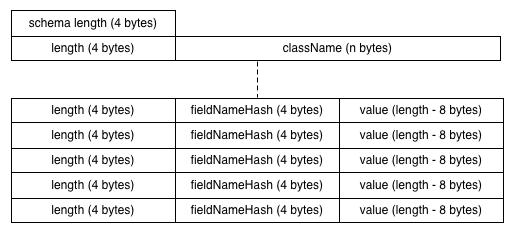
\includegraphics[width=1\textwidth]{schema-reference}
	\caption{The data outline for the serialized data}
	\label{fig:schema-representation}
\end{figure}

% subsection the_serialization_process (end)
% subsection data_serialization (end)
\subsection{Result Serialization} 

% (fold)
\label{sub:result_serialization}

% subsection result_serialization (end)
% section a_framework_for_data_migration (end)
\section{Programmer Responsibilities} 

% (fold)
\label{sec:programmer_responsibilities}

\subsection{Annotation} 

% (fold)
\label{sub:annotation}

% subsection annotation (end)
\subsection{Parallelization} 

% (fold)
\label{sub:parallelization}

% subsection parallelization (end)
% section programmer_responsibilities (end)
\section{The Model} 

% (fold)
\label{sec:the_model}

% section the_model (end)
\section{Exercising the Framework} 

% (fold)
\label{sec:exercising_the_framework}

% section exercising_the_framework (end)
% chapter design_modelling (end)
\chapter{Experimental Results} 

% (fold)
\label{chap:experimental_results}

% chapter experimental_results (end)
\chapter{Conclusion} 

% (fold)
\label{chap:conclusion}

\section{Summary of Contribution} 

% (fold)
\label{sec:summary_of_contribution}

% section summary_of_contribution (end)
\section{Future Work} 

% (fold)
\label{sec:future_work}

% section future_work (end)
% chapter conclusion (end)
%% This changes the headings and chapter titles (no numbers for
%% example).
\backmatter

%% This file is setup to use a bibtex file sample.bib and uses the
%% plain style.  Other styles may be used depending on the conventions
%% of your field of study.
%%
%%% Note: the bibliography must come before the appendices.
\bibliographystyle{plain} 
\bibliography{sample}

%% Use this to reset the appendix counter.  Note that the FoGS
%% requires that the word ``Appendices'' appear in the table of
%% contents either before each appendix lable or as a division
%% denoting the start of the appendices.  We take the latter option
%% here.  This is ensured by making the \texttt{appendicestoc} option
%% a default option to the UBC thesis class.
%%% If you only have one appendix, please uncomment the following line.
% \renewcommand{\appendicesname}{Appendix}
\appendix 
\chapter{First Appendix}
\begin{table}
	\begin{tabular*}{0.75\textwidth}{| c | c | c | } 
		\hline 
			Type & Data Size & Effect On Schema \\
		\hline
			byte or Byte & 1 & 5 \\
		\hline
			char or Character & 2 & 6 \\
		\hline
			short or Short & 2 & 6 \\
		\hline
			float, Float, int, or Integer & 4 & 8 \\
		\hline
			double, Double, long, or Long & 8 & 12 \\
		\hline
			byte[length] & 1 * length & 1 * length + 4 \\
		\hline
			char[length] & 2 * length & 2 * length + 4 \\
		\hline
			float[length] or int[length] & 4 * length & 4 * length + 4 \\
		\hline
			double[length] or long[length] & 8 * length & 8* length + 4 \\
		\hline
			object (not visited) & object.size() & object.size() + 8 \\
		\hline
			object (visited) & object.size() & 8 \\
		\hline
	\end{tabular*}
	\caption{Table of field sizes} 
	\label{tab:field_sizes} 
\end{table}

\chapter{Second Appendix} Here is the second appendix.

\end{document} 
\endinput

%%
%% End of file `ubcsample.tex'.
